% !TEX TS-program = pdflatex
% !TEX encoding = UTF-8 Unicode

\documentclass[11pt]{article}
\usepackage[utf8]{inputenc} 
\usepackage[parfill]{parskip}
\usepackage[T1]{fontenc} 

\usepackage{polski}
\usepackage{float}
\usepackage{fixltx2e}
\usepackage{calc}
\usepackage[export]{adjustbox} % also loads graphicx
\usepackage{makeidx}
\usepackage{multicol}
\usepackage{multirow}
\PassOptionsToPackage{warn}{textcomp}
\usepackage{textcomp}
\usepackage[nointegrals]{wasysym}
\usepackage[table]{xcolor}

\usepackage{csvsimple}

% Font selection
\usepackage[T1]{fontenc}
\usepackage[scaled=.90]{helvet}
\usepackage{courier}
\usepackage{amssymb}
\usepackage{sectsty}

%%% PAGE DIMENSIONS
\usepackage{geometry} % to change the page dimensions
\geometry{a4paper} % or letterpaper (US) or a5paper or....
\geometry{margin=1in} % for example, change the margins to 2 inches all round

\usepackage{graphicx} % support the \includegraphics command and options
\usepackage[parfill]{parskip} % Activate to begin paragraphs with an empty line rather than an indent

%%% PACKAGES
\usepackage{booktabs} % for much better looking tables
\usepackage{array} % for better arrays (eg matrices) in maths
\usepackage{paralist} % very flexible & customisable lists (eg. enumerate/itemize, etc.)
\usepackage{verbatim} % adds environment for commenting out blocks of text & for better verbatim
\usepackage{subfig} % make it possible to include more than one captioned figure/table in a single float
% These packages are all incorporated in the memoir class to one degree or another...
\usepackage{graphicx}

\usepackage{ifpdf}
\ifpdf
\usepackage[pdftex,pagebackref=true]{hyperref}
\else
\usepackage[ps2pdf,pagebackref=true]{hyperref}
\fi
\hypersetup{%
	colorlinks=true,%
	urlcolor=blue,
	linkcolor=blue,%
	citecolor=blue,%
	unicode%
}


%%% HEADERS & FOOTERS
\usepackage{fancyhdr} % This should be set AFTER setting up the page geometry
\pagestyle{fancy} % options: empty , plain , fancy
\renewcommand{\headrulewidth}{0pt} % customise the layout...
\lhead{}\chead{}\rhead{}
\lfoot{}\cfoot{\thepage}\rfoot{}
%%% END Article customizations

%%% The "real" document content comes below...

\title{ConcreteTorrent - Projekt Wstępny}
\author{Jakub Bryl, Bartosz Ciućkowski, Michał Mazurek, Piotr Zmyślony}
\date{6 kwietnia 2020} % Activate to display a given date or no date (if empty),
% otherwise the current date is printed 

\begin{document}
	\maketitle
	\setcounter{secnumdepth}{3}
	\setcounter{tocdepth}{3}
	\tableofcontents
	\clearpage
\section{Treść zadania}
Użytkownik dołącza do sieci \textsl{peer-to-peer} poprzez skontaktowanie się z serwerem, po czym przekazuje serwerowi listę plików jakie jest w stanie udostępnić (może później tę listę edytować). Gdy użytkownik chce pobrać plik, wysyła zapytanie o ten plik do serwera, który zwraca mu listę użytkowników posiadających całość lub część tego pliku. Użytkownik pobierający plik może udostępniać innym użytkownikom tą część pliku, którą udało mu się już pobrać. Podczas pobierania pliku użytkownik będzie cyklicznie odpytywał serwer o to czy w sieci pojawił się ktoś nowy, kto udostępnia pobierany plik. Serwer powinien móc pracować w przestrzeni adresów IPv4 i IPv6.

Krótki słownik pojęć stosowanych w dalszej części dokumentu:
\begin{itemize}
\item \textbf{Tracker} - serwer, z którym łączą się klienci.
\item \textbf{Klient} - aplikacja po stronie użytkownika. Odpowiada za przesyłanie/odbieranie plików oraz za kontaktowanie się z trackerem i z innymi klientami.
\item \textbf{Seed} - klient posiadający kompletny plik.
\item \textbf{Peer} - klient posiadający fragmenty plików, które udostępnia i równocześnie pobiera brakujące fragmenty.
\item \textbf{Segment} - fragment pliku.
\end{itemize}

\section{Założenia funkcjonalne i niefunkcjonalne}
\subsection{Wymagania dotyczące trackera}
Wymagania funkcjonalne:
\begin{enumerate}
\item System powinien oferować usługę serwera (tracker), który koordynuje wymianę plików pomiędzy użytkownikami umożliwiając znajdowanie siebie nawzajem.
\item Sam serwer nie powinien posiadać kopii plików czy ich części.
\item Użytkownik może uruchomić tracker, będący pośrednikiem w wymianie plików pomiędzy innymi użytkownikami.
\end{enumerate}
Wymagania niefunkcjonalne:
\begin{enumerate}
\item Tracker powinien zwracać listę osób, od których użytkownik może pobrać plik w rozsądnym czasie.
\end{enumerate}
\subsection{Wymagania dotyczące klienta}
Wymagania funkcjonalne:
\begin{enumerate}
\item Klient może zawiadomić trackera, o tym, że udostępnia konkretny plik w całości lub w części.
\item Klient może zażądać od trackera listy innych użytkowników udostępniających konkretne pliki.
\item Klient może poprosić innego klienta o wysłanie wybranych fragmentów pliku.
\item Klient może zapytać innego użytkownika o listę fragmentów, jakie posiada.
\item Klient powinien móc równocześnie pobierać i udostępniać zasoby.
\end{enumerate}
Wymagania niefunkcjonalne:
\begin{enumerate}
\item Klient nie powinien mieć problemu z jednoczesnym pobieraniem od 5 osób.
\item Klient powinien móc zamknąć program bez ryzyka utraty pobranych fragmentów.
\item W przypadku awarii fragmenty plików już pobranych powinny być niezagrożone
\end{enumerate}

\section{Podstawowe przypadki użycia}
\subsection{UC1. Użytkownik łączy się z siecią P2P:}
\begin{enumerate}
	\item Użytkownik kontaktuje się z serwerem.
	\item Przekazuje mu listę plików, które posiada i jest gotowy udostępniać
	\item W przypadku, gdy inny użytkownik zażąda któregoś z plików, zacznie mu go od razu udostępniać.
	\item W każdym momencie użytkownik ma również możliwość rozpoczęcia pobierania od innych użytkowników.
\end{enumerate}
Alternatywna ścieżka \textsl{A}:
\begin{itemize}
	\item [3a.] Użytkownik nie posiada żadnego pliku do udostępniania (pusta lista).
	\item [4a.] Serwer nie blokuje użytkownikowi przejścia do kolejnego kroku.
\end{itemize}
\subsection{UC2. Użytkownik chce pobrać określony plik:}
\begin{enumerate}
	\item Użytkownik łączy się z siecią P2P. (UC1.)
	\item Określa jaki plik go interesuje.
	\item Tracker udostępnia listę dostępnych użytkowników posiadających całość lub część pliku.
	\item Użytkownik łączy się z nimi i rozpoczyna pobieranie, jednocześnie udostępniając już posiadane fragmenty (peer).
	\item Po uzyskaniu całości pliku użytkownik nadal udostępnia go innym (seed).

\end{enumerate}
Alternatywna ścieżka \textsl{A}:
\begin{itemize}
	\item [3a.] Serwer nie posiada informacji o żadnym użytkowniku udostępniającym żądany plik.
	\item [4a.] Użytkownik informowany jest o problemie.
	\item [5a.] Użytkownik ma możliwość kolejnego żądania.
\end{itemize}
Alternatywna ścieżka \textsl{B}:
\begin{itemize}
	\item [6b.] Użytkownik kończy połączenie z innymi użytkownikami.
	\item [7b.] Plik znajduje się na urządzeniu użytkownika, ale nie jest dalej przekazywany.
\end{itemize}
\subsection{UC3. Użytkownik chce udostępniać nowy plik (dodać do trackera):}
\begin{enumerate}
	\item Użytkownik przygotowuje specjalny plik zawierający dane o pliku, który zamierza udostępnić innym.
	\item Przesyła plik do wybranego trackera.
	\item Tracker odsyła komunikat o powodzeniu dodania pliku wraz z wygenerowanym unikalnym identyfikatorem.
\end{enumerate}
Alternatywna ścieżka \textsl{A}:
\begin{itemize}
	\item [3a.] Tracker odsyła komunikat o niepowodzeniu wraz z przyczyną.
\end{itemize}
\section{Wybrane środowisko sprzętowo-programowe}
\paragraph{System operacyjny:}
Ubuntu 16.04 i nowsze
\paragraph{Język programowania:}
 C++17
\paragraph{System budowania aplikacji:}
CMake
\paragraph{Biblioteki:}
Google Protocol Buffers, spdlog (\url{github.com/gabime/spdlog})
\paragraph{Testowanie:}
Catch lub Boost.Test (jeszcze do ustalenia), Docker
\section{Architektura rozwiązania}
\begin{figure}[h]
\caption{Schemat komunikacji sieciowej}
\centering
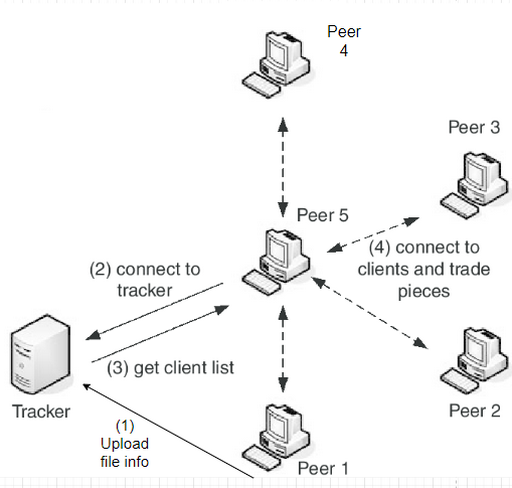
\includegraphics[scale=0.8]{0}
\end{figure}
\clearpage
\subsection{Budowa klienta}
\begin{figure}[h]
\caption{Schemat modułów klienta}
\centering
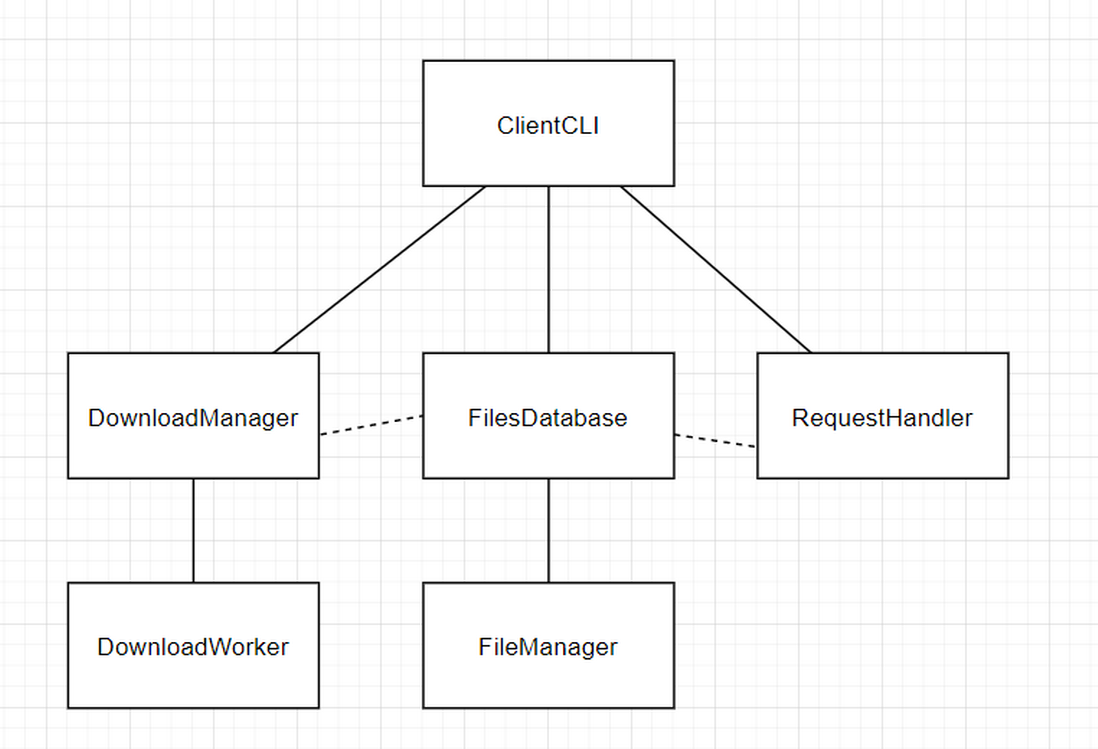
\includegraphics[scale=0.4]{1}
\end{figure}

\textbf{ClientCLI} -- moduł odpowiedzialny za przyjmowanie żądań od użytkownika i przekazywanie ich innym modułom oraz za wyświetlanie informacji użytkownikowi.

\textbf{DownloadManager} -- odpowiada za pobieranie jednego pliku. Tworzy kilka wątków DownloadWorkera, odpowiedzialnych za pobieranie fragmentów danego pliku. DownloadManager kompletuje fragmenty i przesyła je do FilesDatabase.

\textbf{DownloadWorker} -- ma za zadanie znalezienie klienta posiadającego jeden z brakujących fragmentów pliku i nawiązanie z nim połączenia. Po nawiązaniu połączenia, pobiera od niego brakujący fragment i wysyła zapytanie o listę fragmentów, które klient posiada. Jeżeli posiada fragmenty których brakuje, prosi o wysłanie kolejnych fragmentów. 

\textbf{FilesDatabase} -- przechowuje informacje o plikach, które interesują konkretnego klienta (ma taki plik lub jest w trakcie pobierania). Z każdym pobieranym plikiem, przechowywana jest również informacja o klientach posiadających fragmenty danego pliku.

\textbf{FileManager} -- API służące do odczytywania zasobów z systemu plików i buforowania ich oraz do zapisywania na dysku zbuforowanych danych.

\textbf{RequestHandler} -- moduł odbierający i odpowiadający na żądania pobierania fragmentu pliku oraz żądanie o informacje na temat posiadanych fragmentów pliku. 

\clearpage
\subsection{Budowa trackera}
\begin{figure}[h]
\caption{Schemat modułów trackera}
\centering
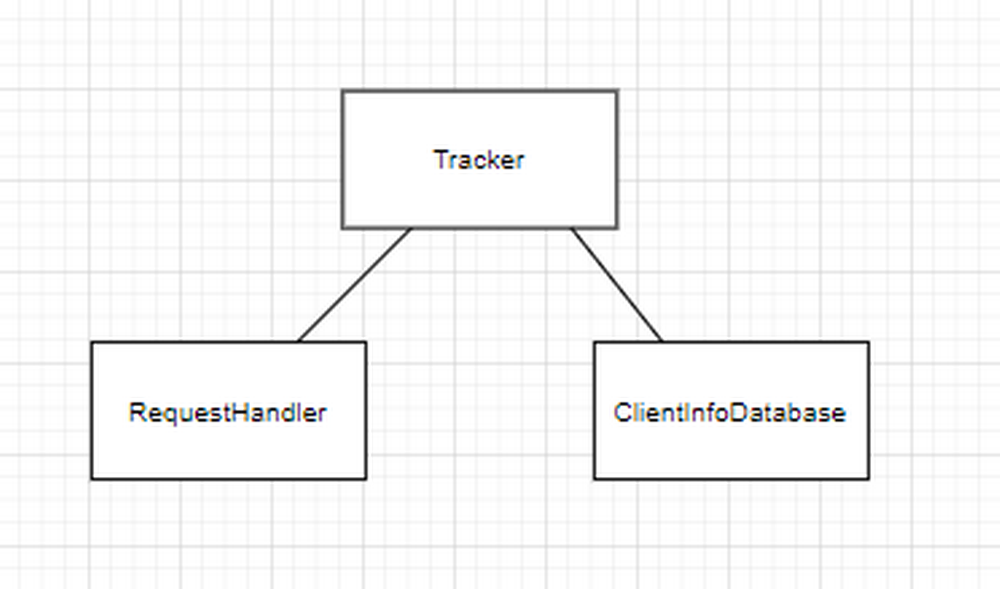
\includegraphics[scale=0.4]{2}
\end{figure}

\textbf{ClientInfoDatabase} - przechowuje informacje o klientach w sieci oraz o posiadanych przez nich plikach.


\textbf{RequestHandler} - odbiera i odpowiada na żądania o listę klientów posiadających dany plik oraz na żądanie udostępnienia pliku w sieci przez klienta.

\section{Lista komunikatów sieciowych}
Komunikacja w naszym systemie będzie zachodziła ścieżkami klient--tracker i klient--klient. Dodatkowo, każdy klient może równolegle komunikować się z wieloma innymi klientami korzystającymi z tego samego trackera.
\subsection{Komunikaty klient--tracker}
\begin{itemize}
\item \textbf{CS\_SEEDLIST\_REQUEST} -- klient wysyła zapytanie do serwera, o to czy jakiś inny klient posiada dany plik w całości lub w części. Komunikat ten sygnalizuje również trackerowi, żeby dodać klienta do listy adresów udostępniających danych plik.
\item \textbf{CS\_SEEDLIST\_RESPONSE} -- jeżeli jacyś klienci faktycznie udostępniają dany plik, tracker odsyła pytającemu adresy tych klientów, wraz z oznaczeniem czy są peerami czy seedami.
\item \textbf{CS\_CLIENT\_UNAVAILABLE} -- komunikat sygnalizujący sytuację, w której klient A dowiedział się od klienta B, że nie udostępnia już danego pliku. W tym wypadku tracker, aby usunąć klienta B z posiadaczy pliku, potrzebuje odebrać więcej podobnych raportów od innych klientów.
\item \textbf{CS\_IM\_A\_SEED} -- klient ogłasza trackerowi, że jest posiadaczem całości pliku.
\item \textbf{CS\_NEW\_REQUEST} -- klient prosi tracker o dodanie posiadanego pliku do listy udostępnianych.
\item \textbf{CS\_NEW\_RESPONSE} -- tracker odpowiada klientowi o sukcesie lub niepowodzeniu dodania pliku do listy udostępnianych.
\end{itemize}

\subsection{Komunikaty klient--klient}
\begin{itemize}
\item \textbf{CC\_LIST\_REQUEST} -- jeden klient \textsl{A} pyta drugiego (klienta \textsl{B}), jakie fragmenty konkretnego pliku/plików posiada.
\item \textbf{CC\_LIST\_RESPONSE} -- odpowiedź do powyższego zapytania. W przypadku udostępniania danego pliku - wysyła listę posiadanych fragmentów (lub tych których nie ma - zależnie od tego których jest mniej). Klient \textsl{B} może odpowiedzieć, że takiego pliku w ogóle nie udostępnia - w tym wypadku klient \textsl{A} wysyła \textsl{CS\_CLIENT\_UNAVAILABLE} do trackera, z którego otrzymał informacje o kliencie \textsl{B}.
\item \textbf{CC\_FRAGMENT\_REQUEST} -- komunikat proszący klienta o przesłanie danego fragmentu pliku.
\item \textbf{CC\_FRAGMENT\_RESPONSE} -- zawiera blok danych (fragment), o który prosił go inny klient. Może również odpowiedzieć, że nie zgadza się na wysłanie tego fragmentu (lub, że już go nie posiada).
\end{itemize}


\section{Sposób testowania}
Zastosujemy testy jednostkowe, sprawdzające poprawność działania pojedynczych części systemu, tworzone przy użyciu odpowiednich bibliotek wymienionych powyżej.

Do tego planujemy utworzyć skrypty testowe symulujące realne użycie z pomocą narzędzia \textsl{Docker}. Pozwoli ono przetestować działanie naszego systemu na indywidualnych maszynach poprzez utworzenie sieci kontenerów, symulujących większą ilość klientów i trackerów.

\newcommand{\RomanNumeralCaps}[1]
    {\MakeUppercase{\romannumeral #1}}
\section{Sposób demonstracji rezultatów}
Wyróżniliśmy następujące scenariusze testowe:
\paragraph{Scenariusz \RomanNumeralCaps{1}} Podłączenie się przez użytkownika \textsl{A} do systemu i przekazanie trackerowi informacji o posiadanym pliku. Następnie podłączenie do systemu użytkownika \textsl{B} i zażądanie od trackera informacji o klientach posiadających wysłany przez \textsl{A} plik. Tracker powinien zwrócić klientowi \textsl{B} adres klienta \textsl{A}. Następnie \textsl{B} wysyła do \textsl{A} prośby o kolejne segmenty pliku, \textsl{A} mu je odsyła, aż do skompletowania całego pliku.
\paragraph{Scenariusz \RomanNumeralCaps{2}} Scenariusz podobny jak wyżej, ale z większą liczbą użytkowników posiadających dany plik. Test ten pokaże pobieranie współbieżne od kilku klientów.
\paragraph{Scenariusz \RomanNumeralCaps{3}} Dwóch klientów (\textsl{A} i \textsl{B}) udostępniających po jednym pliku, odpowiednio \textsl{P1} i \textsl{P2}. Test ten zaprezentować ma pobieranie przez \textsl{A} pliku \textsl{P2} od \textsl{B} oraz pobieranie przez \textsl{B} pliku \textsl{P2} od \textsl{A}.
\paragraph{Scenariusz \RomanNumeralCaps{4}} Klient jest w trakcie pobierania pliku. Proces klienta zostaje nagle zamknięty i włączony ponownie. Test zakończy się sukcesem, jeśli klient wznowi pobieranie pliku, bez utraty fragmentów pobranych przed wyłączeniem.

\clearpage
\section{Organizacja pracy}
\subsection{Podział pracy}
Podział prac jest bardzo orientacyjny i z łatwością może ulec zmianie, ponieważ nie jesteśmy pewni ile nakładu pracy będą wymagały poszczególne moduły. Wstępny podział wygląda następująco:
\begin{itemize}
\item \textbf{DownloadManager}, \textbf{DownloadWorker}, \textbf{FilesDatabase} i \textbf{ClientInfoDatabase} -- Jakub Bryl, Michał Mazurek
\item \textbf{RequestHandlers}, \textbf{ClientCLI} i \textbf{FileManager} -- Piotr Zmyślony, Bartosz Ciućkowski 
\end{itemize}
\subsection{Harmonogram}
Główne kamienie milowe i terminy:

\textbf{27 kwietnia} - Wymiana informacji między klientem a trackerem oraz podstawowa komunikacja między klientami. 

\textbf{12 maja} - Współbieżna wymiana plików między wieloma klientami. 

\subsection{Zdalne repozytoria}
Projekt jest rozwijany przy pomocy systemu kontroli wersji git, pod adresem \url{https://github.com/zmysloony/p2p-network/}. Dodatkowo korzystamy z Trello do zarządzania zadaniami i wymiany pomysłów: \url{https://trello.com/b/EuSrukdO/tin-torrent}.
\end{document}